\documentclass[10pt,letterpaper]{article}
\usepackage[T1]{fontenc}
\usepackage[utf8]{inputenc}
\usepackage{lmodern}
\usepackage[margin=0.78in,headheight=14pt]{geometry}
\usepackage{microtype}
\usepackage{amsmath,amssymb}
\usepackage{booktabs,tabularx,longtable,array}
\usepackage{enumitem}
\usepackage{xcolor,tikz}
\usetikzlibrary{arrows.meta,positioning,calc,fit,shapes.geometric}
\usepackage{listings}
\usepackage{caption}
\usepackage{fancyhdr}
\usepackage{xurl}
\usepackage{hyperref}
\hypersetup{colorlinks=true,linkcolor=blue!45!black,urlcolor=blue!45!black,
 pdftitle={OpenRocket MIT: Flight-computer API and architecture},
 pdfauthor={OpenRocket MIT development documentation},bookmarksnumbered=true}
\definecolor{ink}{HTML}{17334A}
\definecolor{accent}{HTML}{007B91}
\definecolor{pale}{HTML}{EEF5F9}
\definecolor{muted}{HTML}{526779}
\definecolor{warm}{HTML}{FFF6DD}
\pagestyle{fancy}
\fancyhf{}
\fancyhead[L]{\small\sffamily\color{muted}OPENROCKET MIT / FLIGHT COMPUTER}
\fancyhead[R]{\small\sffamily\color{muted}6.4}
\fancyfoot[L]{\small\sffamily Architecture and implementation contracts}
\fancyfoot[R]{\small\sffamily\thepage}
\renewcommand{\headrulewidth}{0.3pt}
\setlength{\parindent}{0pt}
\setlength{\parskip}{6pt}
\setlength{\emergencystretch}{2em}
\setlist{nosep,leftmargin=1.4em,topsep=4pt}
\renewcommand{\arraystretch}{1.18}
\captionsetup{font=small,labelfont={bf,color=ink},skip=8pt}
\newcolumntype{Y}{>{\raggedright\arraybackslash}X}
\newcommand{\code}[1]{\nolinkurl{#1}}
\newcommand{\class}[1]{\nolinkurl{#1}}
\newcommand{\us}{\ensuremath{\,\mu\mathrm{s}}}
\newcommand{\ms}{\ensuremath{\,\mathrm{ms}}}
\newcommand{\api}[2]{\href{javadoc/#1.html}{\texttt{#2}}}
\lstset{basicstyle=\ttfamily\small,breaklines=true,columns=fullflexible,
 keepspaces=true,frame=single,rulecolor=\color{accent!35},backgroundcolor=\color{pale},
 xleftmargin=6pt,xrightmargin=6pt,aboveskip=8pt,belowskip=8pt,showstringspaces=false}
\tikzset{
 box/.style={draw=ink!75,fill=pale,rounded corners=2pt,align=left,
 inner sep=6pt,font=\fontsize{8}{10}\selectfont,minimum height=0.85cm},
 group/.style={draw=accent!45,dashed,rounded corners=3pt,inner sep=8pt},
 use/.style={-{Latex[length=5pt]},draw=ink!80,line width=0.55pt},
 inherit/.style={-{Triangle[open,length=7pt,width=6pt]},draw=ink!80,line width=0.6pt},
 own/.style={{Diamond[fill=ink,length=6pt,width=4pt]}-,draw=ink!80,line width=0.6pt},
 flowlabel/.style={font=\fontsize{7.5}{9}\selectfont,fill=white,inner sep=2pt,align=center},
 note/.style={draw=accent!30,fill=warm,rounded corners=2pt,align=left,inner sep=6pt,
 font=\fontsize{8}{10}\selectfont},
 lifeline/.style={draw=muted!65,densely dashed},
 participant/.style={box,align=center,minimum height=1cm,font=\fontsize{8}{10}\selectfont}
}
\newcommand{\uml}[5]{\node[box,text width=#5] (#1) at (#2)
 {\centering\bfseries\ttfamily #3\par\vspace{2pt}\hrule\vspace{3pt}
 \raggedright\normalfont\ttfamily #4};}
\newcommand{\simple}[4]{\node[box,text width=#4,align=center] (#1) at (#2)
 {\bfseries\ttfamily #3};}
\newcommand{\diagram}[3]{\begin{figure}[htbp]\centering
\resizebox{\linewidth}{!}{#3}\caption{#2}\label{#1}\end{figure}}
\begin{document}
\begin{titlepage}
\color{ink}
{\sffamily\bfseries\Large OPENROCKET MIT\par}
\vspace{1.25cm}
{\sffamily\bfseries\Huge Flight-computer API\par}
\vspace{0.2cm}
{\sffamily\bfseries\Huge and architecture\par}
\vspace{0.55cm}
{\Large Namespace refactor, runtime contracts and framework integration\par}
\vspace{0.7cm}
{\large Edition 6.4\quad /\quad 11 October 2026\par}
\vspace{0.8cm}
\hrule height 1pt
\vspace{0.5cm}
\textbf{The runtime namespace is now \code{edu.mit.rocket_team}.}
The functional subpackages remain intact. The main translated sketch is
\code{edu.mit.rocket_team.FC.RTFC}.

This report describes the implementation, the OpenRocket engine connections,
measurement and clock contracts, controller ownership, recovery, telemetry,
the graphical designer, and surrounding simulation improvements.
All diagrams, tables and equations are native LaTeX; the diagrams are drawn
with TikZ in this self-contained source file. No external figures are required.
\par
\vspace{0.65cm}
\begin{tabularx}{\linewidth}{@{}>{\bfseries}p{3.4cm}Y@{}}
\toprule
Refactor scope & 150 pre-existing Java files: the full firmware translation and the files introduced by the MIT improvements.\\
Documentation & 1,560 explicit methods and constructors documented, including the new six-method audit utility.\\
Verification & 148 core tests and 65 Swing/UI tests passed; the root application JAR was rebuilt.\\
Architecture & Nine UML and sequence views; all 36 top-level firmware classes are indexed.\\
\bottomrule
\end{tabularx}
\vfill
{\small\color{muted}The report records software behavior and verified virtual-time contracts.
It does not qualify physical flight hardware, processor execution time,
inter-board communications or actuator dynamics.}\par
\end{titlepage}
\setcounter{tocdepth}{1}
{\small\setlength{\parskip}{0pt}
\tableofcontents
\vspace{0.15cm}
\listoffigures
}
\clearpage

\section{Scope and namespace migration}
The former \code{edu.mit.rocket_team.zephyrus} root has become
\code{edu.mit.rocket_team}. Subpackages such as \code{FC}, \code{instrument},
\code{control} and \code{telemetry} remain. The change updates source paths,
package declarations, imports, module exports, tests and live documentation references.

\begin{lstlisting}[language=Java]
// Previous: edu.mit.rocket_team.zephyrus.FC.RTFC
import edu.mit.rocket_team.FC.RTFC;
\end{lstlisting}

There is no compatibility package at the old namespace. External source that
imports these firmware classes must update its imports, and compiled clients
must be rebuilt. Custom boards using the supported API
\code{info.openrocket.core.simulation.flightcomputer.JavaBoardProgram}
do not require an import change.

Firmware model identifiers, \code{.fc} schema versions, telemetry byte layouts,
existing log prefixes and the extension class \class{ZephyrusFlightComputer}
retain their identities. Saved design and simulation-extension references can
therefore continue to load. Historical benchmark logs retain their meaning as
records of the builds that produced them.

\subsection{Readability and documentation coverage}
The source manifest covers the translated firmware and Java files introduced
for the FC designer, controller blocks, physical actuator and recovery bridges,
sensor models, telemetry replay, ensembles, motor batches, 3D plotting,
update/memory helpers, tests and standalone verification tools.

Methods use consistent four-space formatting with blank-line separation.
Every explicit method and constructor in that manifest has a Javadoc description,
including private helpers and anonymous-class callbacks. Compiler-generated
record accessors and implicit constructors are not explicit source declarations.

Selected pre-existing OpenRocket integration classes are included in the
browsable reference for context. They are outside the newly documented-method
coverage requirement; malformed comments and stale links encountered during
Javadoc generation were repaired. The application runtime did not acquire a
new documentation dependency.

\subsection{Behavior preservation and reading the diagrams}
The parser comparison found identical executable token streams in all 150
original scoped files after ignoring comments/formatting and normalizing the
namespace. This comparison concerns this refactor; previously implemented
controller and recovery features retain their own functional changes.

Class diagrams show selected operations rather than reproducing the entire
API. A hollow triangle points to a superclass or interface; a filled diamond
marks an owning runtime relationship; ordinary arrows denote use or data flow.
Sequence diagrams describe virtual ordering, not desktop wall-clock latency.
The full method reference is generated in \code{doc/improvements/javadoc/}.

\clearpage
\section{Connection to the OpenRocket engine}
\class{Simulation} selects an engine. Both \class{BasicEventSimulationEngine}
and \class{ModifiedEventSimulationEngine} use the existing listener lifecycle
and advance a physical stepper. \class{SimulationStatus} carries physical state,
conditions, active components and the result branch. The FC extension freezes
and validates its external design, checks custom Java approval and installs
one \class{FlightControllerSimulatorListener}.

\diagram{fig:engine}{Engine integration. The existing extension and listener connect the renamed runtime to the physical simulation.}{%
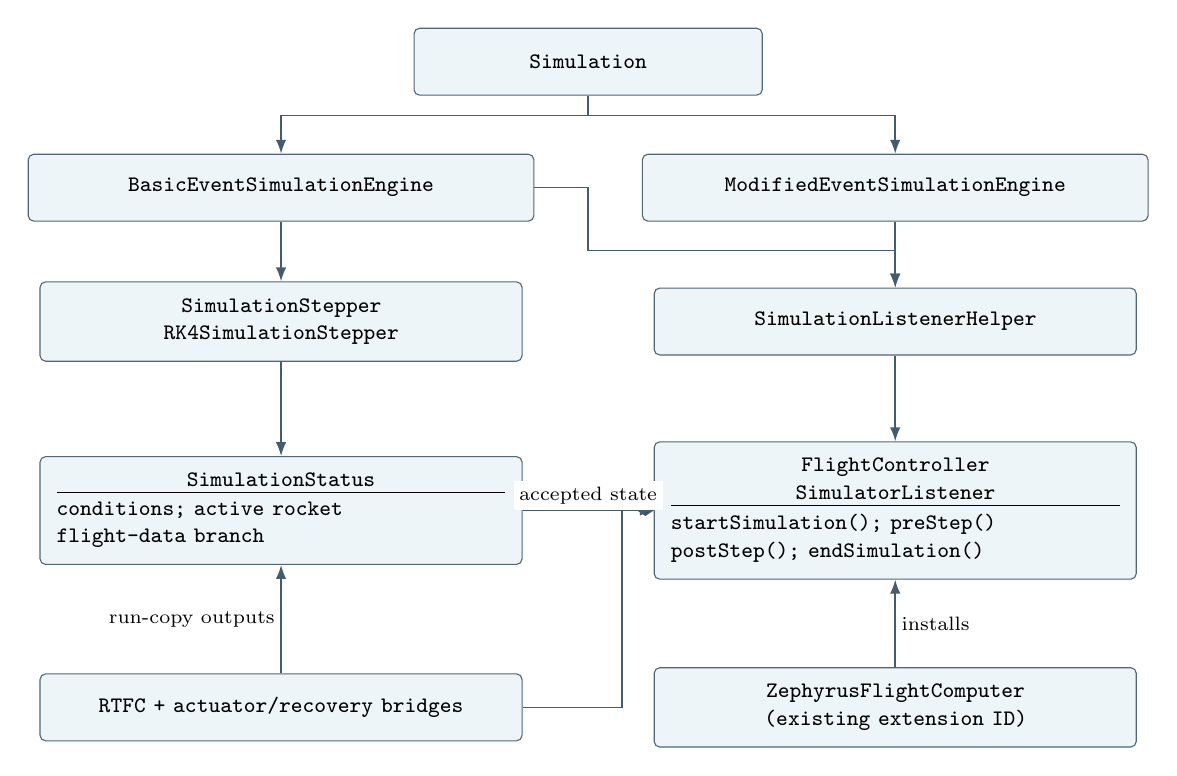
\begin{tikzpicture}
\simple{sim}{7.7,0}{Simulation}{4cm}
\simple{basic}{3.8,-1.6}{BasicEventSimulationEngine}{6cm}
\simple{modified}{11.6,-1.6}{ModifiedEventSimulationEngine}{6cm}
\simple{step}{3.8,-3.3}{SimulationStepper\\RK4SimulationStepper}{5.7cm}
\simple{helper}{11.6,-3.3}{SimulationListenerHelper}{5.7cm}
\uml{status}{3.8,-5.7}{SimulationStatus}{conditions; active rocket\\flight-data branch}{5.7cm}
\uml{listener}{11.6,-5.7}{FlightController\\SimulatorListener}{startSimulation(); preStep()\\postStep(); endSimulation()}{5.7cm}
\simple{ext}{11.6,-8.2}{ZephyrusFlightComputer\\(existing extension ID)}{5.7cm}
\simple{fc}{3.8,-8.2}{RTFC + actuator/recovery bridges}{5.7cm}
\draw[use] (sim.south) -- ++(0,-0.25) -| (basic.north);
\draw[use] (sim.south) -- ++(0,-0.25) -| (modified.north);
\draw[use] (basic) -- (step);
\draw[use] (modified) -- (helper);
\draw[use] (basic.east) -- (7.7,-1.6) -- (7.7,-2.4) -| (helper.north);
\draw[use] (step) -- (status);
\draw[use] (helper) -- (listener);
\draw[use] (ext) -- node[flowlabel,right]{installs} (listener);
\draw[own] (listener.west) -- ++(-0.4,0) |- (fc.east);
\draw[use] (status.east) -- node[flowlabel,above]{accepted state} (listener.west);
\draw[use] (fc) -- node[flowlabel,left]{run-copy outputs} (status);
\end{tikzpicture}}

The listener creates a fresh \class{RTFC}, per-run context, telemetry outputs
and physical bindings. Servo and cant changes apply to the simulation's rocket
copy, preserving the user's design. \code{preStep} limits the next physical
step to a virtual deadline. Coherent accepted acceleration/status samples feed
acquisition; intermediate or future states are not replayed as earlier sensor
measurements. \code{postStep} advances due work and synchronizes FC/physical
result channels. Run shutdown closes outputs and pending recovery work.
The separate \class{AirbrakesControllerListener} is not part of this FC path.

\clearpage
\section{Per-run runtime composition}
\class{RTFC} owns the translated instruments and firmware controllers.
Design-defined state graphs, controller blocks and Java boards extend that
runtime. \class{RTFC.Inputs} carries engineering-unit acquisitions and their
timestamps. \class{RTFC.Output} is the PWM-latched snapshot, including legacy
channels, named servo maps and per-controller outputs.

\diagram{fig:runtime}{Run-local state and the boundaries between acquisitions, task execution and latched outputs.}{%
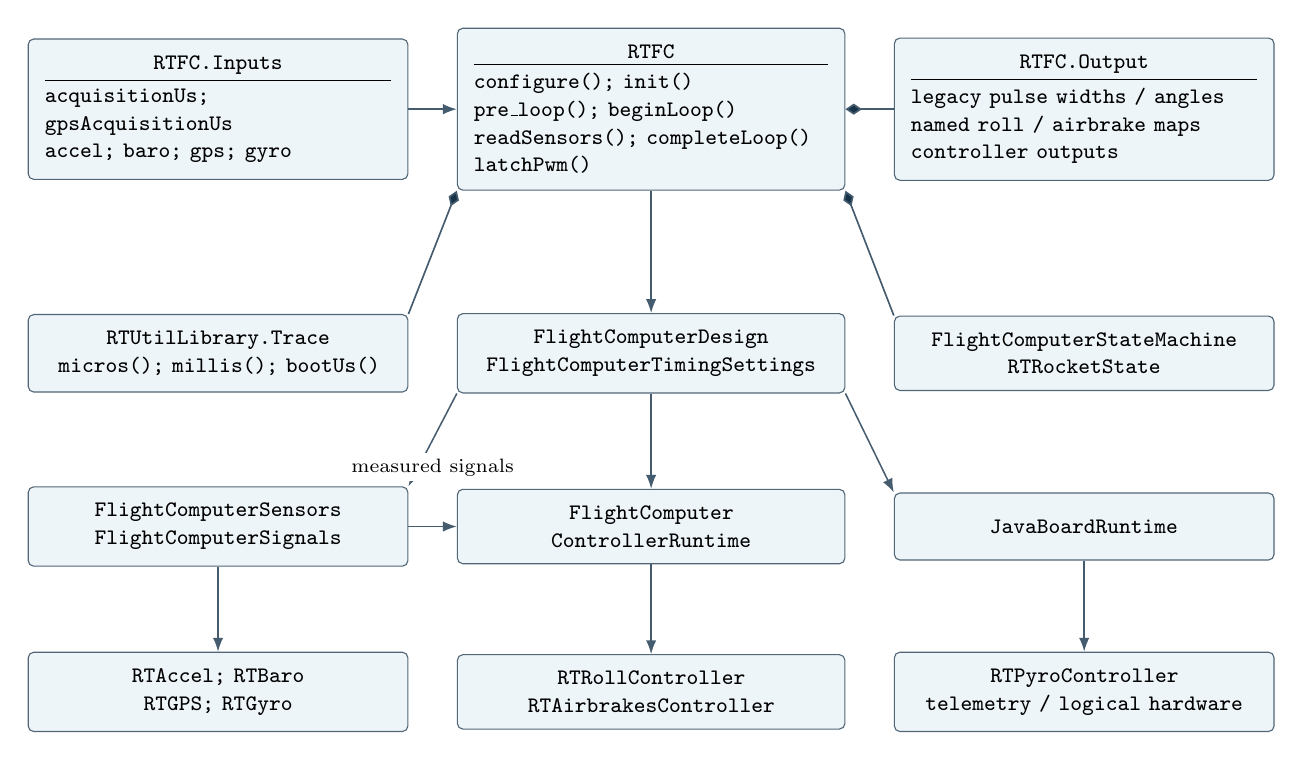
\begin{tikzpicture}
\uml{inputs}{2.5,0}{RTFC.Inputs}{acquisitionUs; gpsAcquisitionUs\\accel; baro; gps; gyro}{4.4cm}
\uml{fc}{8,0}{RTFC}{configure(); init()\\pre\_loop(); beginLoop()\\readSensors(); completeLoop()\\latchPwm()}{4.5cm}
\uml{out}{13.5,0}{RTFC.Output}{legacy pulse widths / angles\\named roll / airbrake maps\\controller outputs}{4.4cm}
\simple{clock}{2.5,-3.1}{RTUtilLibrary.Trace\\micros(); millis(); bootUs()}{4.4cm}
\simple{design}{8,-3.1}{FlightComputerDesign\\FlightComputerTimingSettings}{4.5cm}
\simple{state}{13.5,-3.1}{FlightComputerStateMachine\\RTRocketState}{4.4cm}
\simple{sensors}{2.5,-5.3}{FlightComputerSensors\\FlightComputerSignals}{4.4cm}
\simple{blocks}{8,-5.3}{FlightComputer\\ControllerRuntime}{4.5cm}
\simple{boards}{13.5,-5.3}{JavaBoardRuntime}{4.4cm}
\simple{inst}{2.5,-7.4}{RTAccel; RTBaro\\RTGPS; RTGyro}{4.4cm}
\simple{control}{8,-7.4}{RTRollController\\RTAirbrakesController}{4.5cm}
\simple{services}{13.5,-7.4}{RTPyroController\\telemetry / logical hardware}{4.4cm}
\draw[use] (inputs) -- (fc);
\draw[own] (fc) -- (out);
\draw[own] (fc.south west) -- (clock.north east);
\draw[use] (fc) -- (design);
\draw[own] (fc.south east) -- (state.north west);
\draw[use] (design.south west) -- (sensors.north east);
\draw[use] (design) -- (blocks);
\draw[use] (design.south east) -- (boards.north west);
\draw[use] (sensors) -- (inst);
\draw[use] (blocks) -- (control);
\draw[use] (boards) -- (services);
\draw[use] (sensors.east) -- node[flowlabel,above=16pt]{measured signals} (blocks.west);
\end{tikzpicture}}

The trace is a virtual boot clock and action sink shared by the run's devices.
Sensor histories, task instances, controller state and channel caches belong
to the run. A new simulation receives fresh instances. Physical comparison
curves are recorded separately from the measurements used by controllers.
Logical commands and PWM-latched physical commands are separate states.

\clearpage
\section{Timing contracts}
Boot timestamps are integer microseconds. Physical simulation time zero
follows \(1{,}000{,}000\us\) of virtual warm-up. The preflight command is queued
at \(500{,}000\us\) during warm-up. Firmware \code{micros()} and \code{millis()}
retain unsigned 32-bit wrap; the trace additionally stores unwrapped boot time.
For clocks in the same units, the firmware elapsed-time operation is
\begin{equation}
 \Delta t_{32}=(t_{\mathrm{now}}-t_{\mathrm{then}})\bmod 2^{32}.
\end{equation}

\begin{table}[htbp]\centering\small
\begin{tabularx}{\linewidth}{@{}p{3.1cm}Y@{}}\toprule
Boundary & Implemented contract\\\midrule
FC loop & Nominal 10,000\us\ period, with modeled sensor-read cost, extra work and seeded execution jitter. Loop phases cannot overlap.\\
Held acquisition & Input acquisition and availability times are distinct. A loop uses its held acquisition; GPS retains the original fix timestamp.\\
Independent tasks & Java boards and controller blocks freeze inputs at start, publish at completion and follow independent periods and execution costs.\\
PWM & Commands latch every 20,000\us\ with configurable phase. A task completing exactly on an interrupt boundary misses that latch.\\
State epochs & State changes invalidate work begun in an earlier state; explicit controller-close actions invalidate pending block work.\\
Recovery & Accepted commands retain completion time in microseconds. Physical deployment deadlines do not wait for servo PWM or radio delivery.\\
\bottomrule\end{tabularx}
\caption{Virtual contracts enforced by the existing listener scheduler.}
\end{table}

The firmware's nominal wait is millisecond-quantized. For loop start \(s_n\)
and completion \(c_n\), both in boot microseconds,
\begin{equation}
 s_{n+1}=\max\!\left(c_n,\;1000\left(\left\lfloor\frac{s_n}{1000}\right\rfloor+10\right)\right).
\end{equation}
A custom board or controller block instead uses its own configured period
\(P\):
\begin{equation}
 s_{n+1}=\max(s_n+P,\;c_n).
\end{equation}
An overrun delays the next invocation; it does not create overlapping calls
or a catch-up burst. A faster task does not create fresher measurements.

These are virtual-time contracts. The desktop's elapsed execution time is
not the modeled processor time. Execution costs remain supplied approximations;
board grouping does not simulate shared CPU arbitration or communications
contention between physical boards.

\clearpage
\subsection{Dispatch ordering and the PWM completion tie}
At a coincident boundary, PWM latching precedes FC completion, then controller
and Java-board work. Figure~\ref{fig:scheduler} shows the relevant ordering;
GPS availability and other due services remain part of the same dispatcher.

\diagram{fig:scheduler}{Virtual scheduling: a command completed at the PWM instant is available only after that instant's latch.}{%
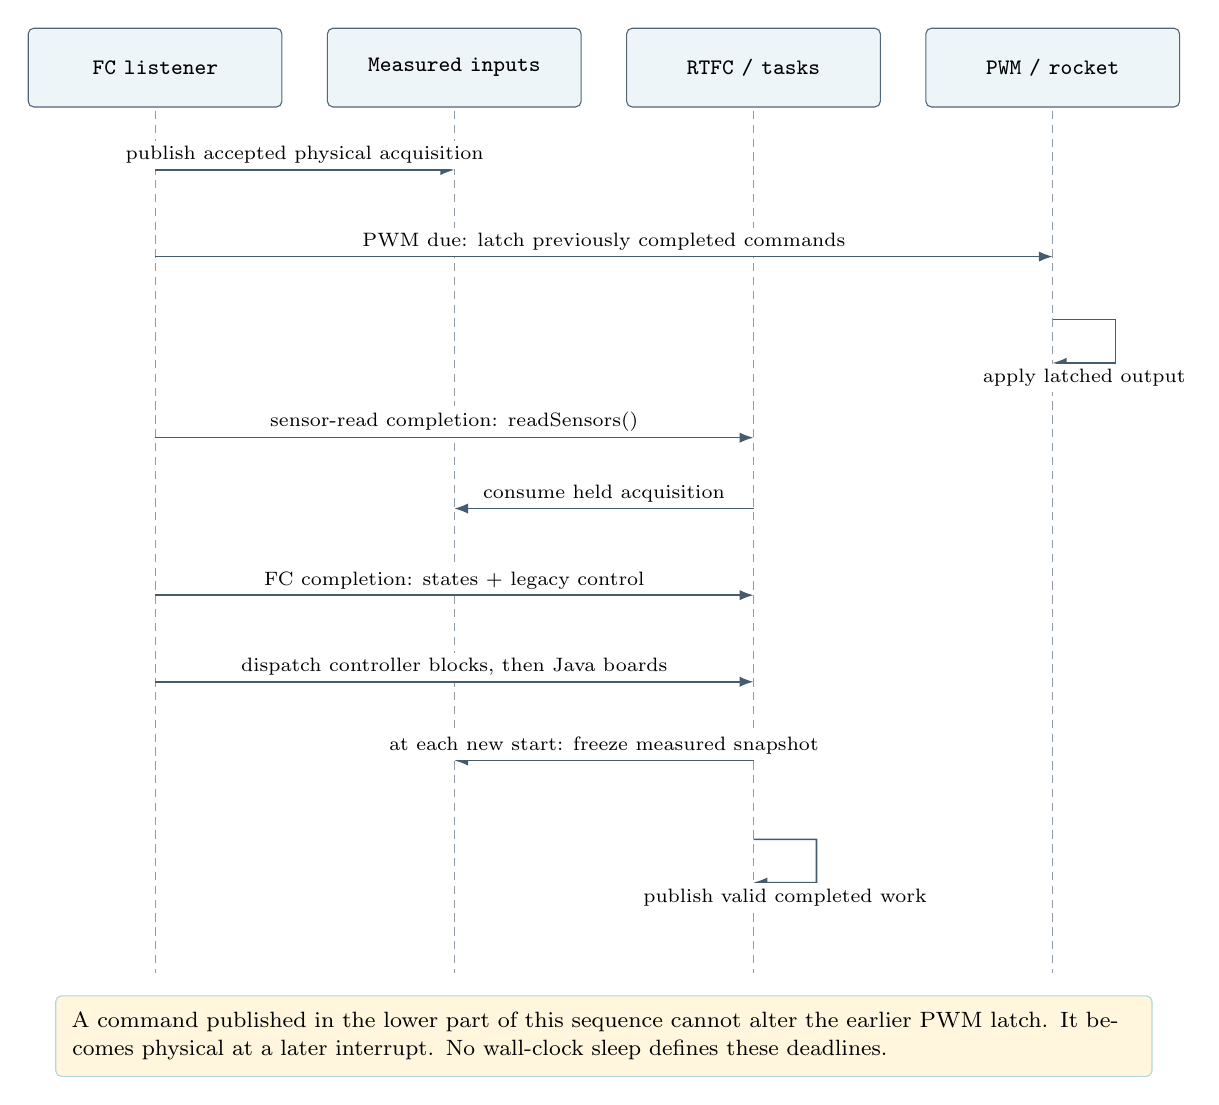
\begin{tikzpicture}
\node[participant,text width=2.8cm] (l) at (1.5,0) {\ttfamily FC listener};
\node[participant,text width=2.8cm] (s) at (5.3,0) {\ttfamily Measured inputs};
\node[participant,text width=2.8cm] (f) at (9.1,0) {\ttfamily RTFC / tasks};
\node[participant,text width=2.8cm] (p) at (12.9,0) {\ttfamily PWM / rocket};
\foreach \x in {1.5,5.3,9.1,12.9} \draw[lifeline] (\x,-0.55) -- (\x,-11.5);
\draw[use] (1.5,-1.3) -- node[flowlabel,above]{publish accepted physical acquisition} (5.3,-1.3);
\draw[use] (1.5,-2.4) -- node[flowlabel,above]{PWM due: latch previously completed commands} (12.9,-2.4);
\draw[use] (12.9,-3.2) -- ++(0.8,0) -- ++(0,-0.55) -- node[flowlabel,below]{apply latched output} (12.9,-3.75);
\draw[use] (1.5,-4.7) -- node[flowlabel,above]{sensor-read completion: readSensors()} (9.1,-4.7);
\draw[use] (9.1,-5.6) -- node[flowlabel,above]{consume held acquisition} (5.3,-5.6);
\draw[use] (1.5,-6.7) -- node[flowlabel,above]{FC completion: states + legacy control} (9.1,-6.7);
\draw[use] (1.5,-7.8) -- node[flowlabel,above]{dispatch controller blocks, then Java boards} (9.1,-7.8);
\draw[use] (9.1,-8.8) -- node[flowlabel,above]{at each new start: freeze measured snapshot} (5.3,-8.8);
\draw[use] (9.1,-9.8) -- ++(0.8,0) -- ++(0,-0.55) -- node[flowlabel,below]{publish valid completed work} (9.1,-10.35);
\node[note,text width=13.5cm] at (7.2,-12.3) {A command published in the lower part of this sequence cannot alter the earlier PWM latch. It becomes physical at a later interrupt. No wall-clock sleep defines these deadlines.};
\end{tikzpicture}}

Task completion must also belong to the current state epoch. Work invalidated
by a state change cannot publish stale control output. The engine's next
physical step is capped at the next pending virtual deadline so the scheduler
does not recreate missed loop ticks using future physical samples.

\clearpage
\section{Measurements and coordinate conventions}
\class{FlightComputerSensors} applies configured mounting rotation, bias,
acquisition cadence and seeded Gaussian noise to accepted simulator inputs.
\class{FlightComputerSignals} publishes stable source IDs, channel descriptors,
validity and acquisition/availability times. Primary sensors retain firmware
filtering and integration; additional sensors keep independent histories.

\diagram{fig:sensors}{Instrument adapters and injected payloads. Hollow triangles identify the two shared base classes.}{%
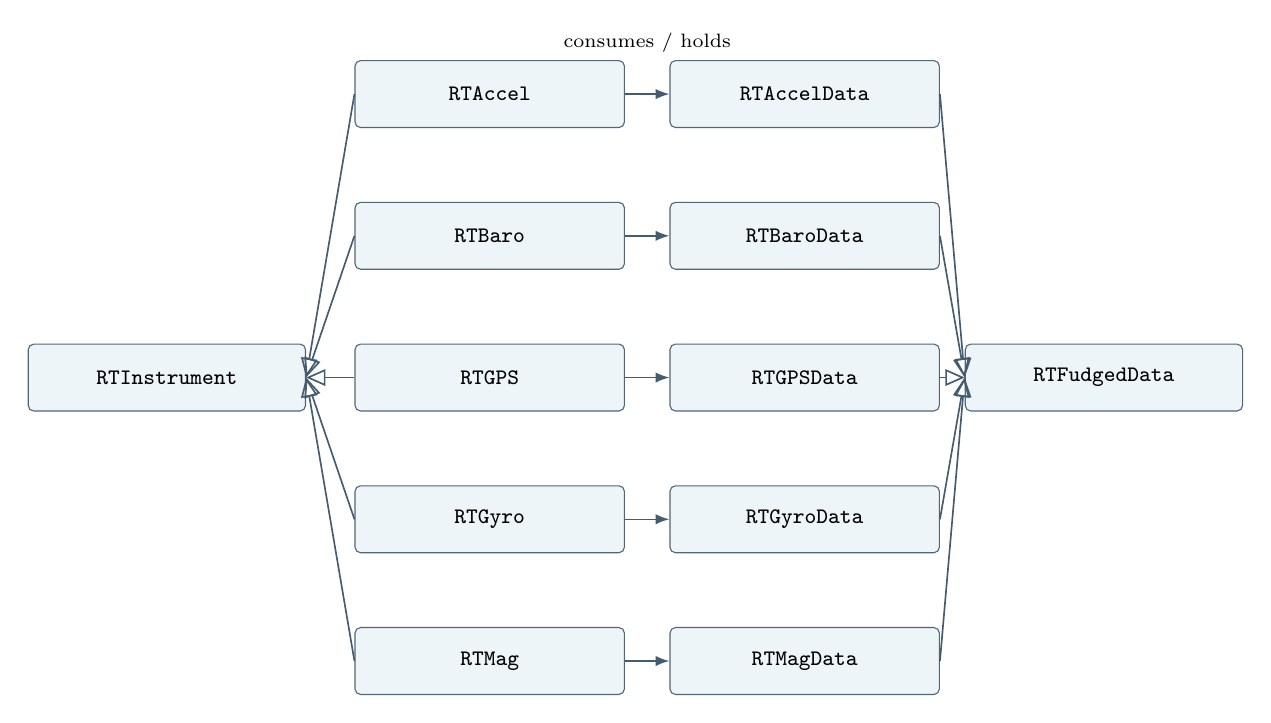
\begin{tikzpicture}
\simple{base}{1.9,-3.6}{RTInstrument}{3.1cm}
\simple{payload}{13.8,-3.6}{RTFudgedData}{3.1cm}
\foreach \name/\data/\yy in {RTAccel/RTAccelData/0,RTBaro/RTBaroData/-1.8,RTGPS/RTGPSData/-3.6,RTGyro/RTGyroData/-5.4,RTMag/RTMagData/-7.2} {
 \simple{\name}{6.0,\yy}{\name}{3cm}
 \simple{\data}{10.0,\yy}{\data}{3cm}
 \draw[inherit] (\name.west) -- (base.east);
 \draw[use] (\name.east) -- (\data.west);
 \draw[inherit] (\data.east) -- (payload.west);
}
\node[flowlabel] at (8,0.65) {consumes / holds};
\end{tikzpicture}}

\begin{table}[htbp]\centering\small
\begin{tabularx}{\linewidth}{@{}p{2.4cm}Y@{}}\toprule
Quantity & Interface convention\\\midrule
Acceleration & Specific force in m/s\(^2\); FC sensor X is OpenRocket body Z. The legacy velocity estimate integrates sensor X minus gravity, rather than ground-speed magnitude or airspeed.\\
Angular rate & Sensor rates in degrees/s. Roll integrates negative sensor X; pitch/yaw use the corresponding held rates.\\
Barometer & Pressure in hPa, temperature in Celsius and height in metres. Pressure altitude passes through the moving average and zero reference.\\
GPS & Input coordinates are decimal degrees and altitude is MSL metres; quantization is \(10^{-7}\) degrees and millimetres. The adapter's \code{getHeight()} and \code{getAltitude()} return zero-relative height.\\
Raw counts & Pressure/temperature ADC counts may be NaN when unavailable. Engineering observations do not imply a modeled electrical sensor bus.\\
\bottomrule\end{tabularx}
\caption{Units at the measured-input boundary.}
\end{table}
Controllers consume measurements; simulator truth is a separate diagnostic
series. Re-reading a held signal does not draw fresh noise. \class{RTMag}
is a legacy adapter outside the active FC measurement loop.

\clearpage
\section{Firmware controllers and physical outputs}
The translated roll controller retains its aerodynamic gain schedule and
elapsed-time PID behavior. The airbrake controller retains the FC-included
coast predictor and state sequence, including integer flight seconds and the
source integral convention. Generic controller-block PID does not replace
these legacy laws.

\diagram{fig:controllers}{Firmware controller hierarchy and the physical bridge. The predictor owns its fit samples; recovery uses a separate event bridge.}{%
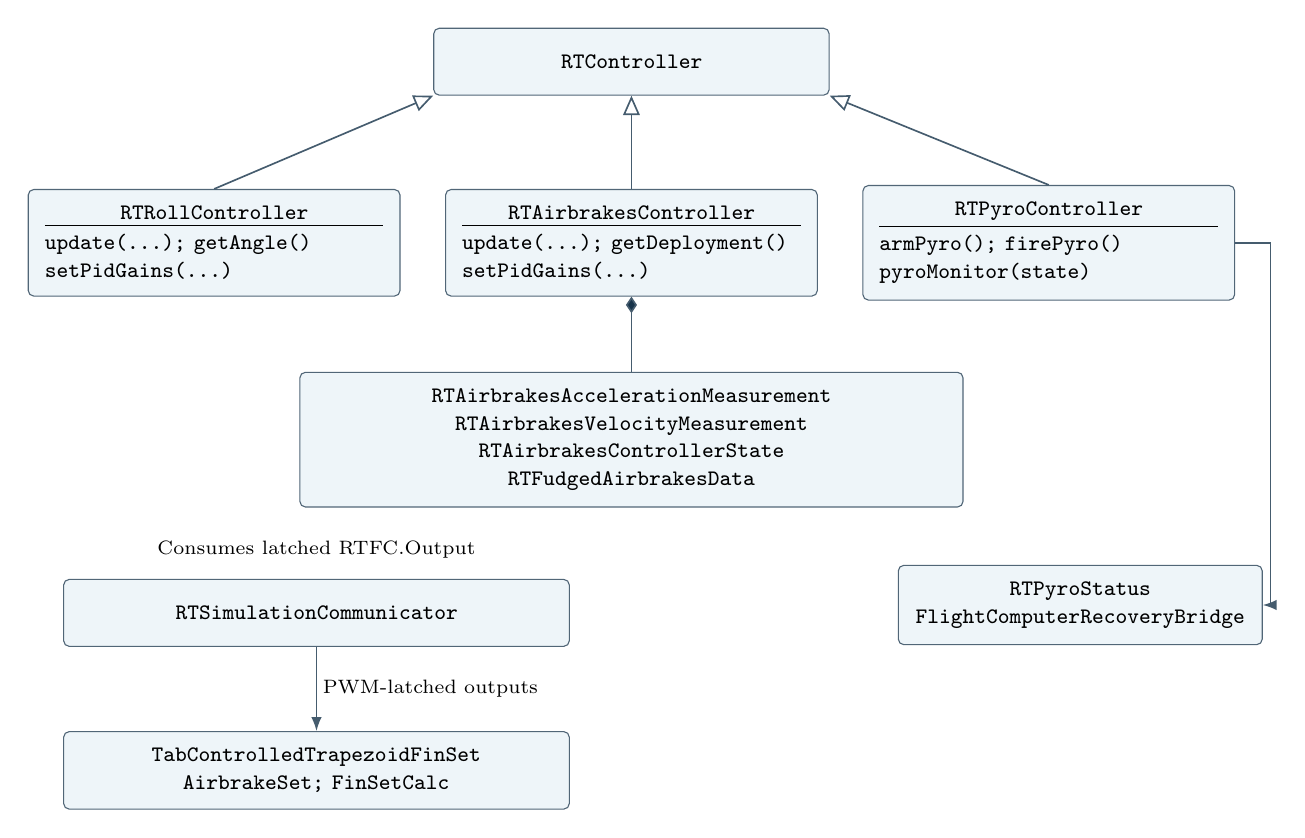
\begin{tikzpicture}
\simple{base}{7.8,0}{RTController}{4.6cm}
\uml{roll}{2.5,-2.3}{RTRollController}{update(...); getAngle()\\setPidGains(...)}{4.3cm}
\uml{brakes}{7.8,-2.3}{RTAirbrakesController}{update(...); getDeployment()\\setPidGains(...)}{4.3cm}
\uml{pyro}{13.1,-2.3}{RTPyroController}{armPyro(); firePyro()\\pyroMonitor(state)}{4.3cm}
\draw[inherit] (roll.north) -- (base.south west);
\draw[inherit] (brakes.north) -- (base.south);
\draw[inherit] (pyro.north) -- (base.south east);
\simple{samples}{7.8,-4.8}{RTAirbrakesAccelerationMeasurement\\RTAirbrakesVelocityMeasurement\\RTAirbrakesControllerState\\RTFudgedAirbrakesData}{8cm}
\draw[own] (brakes) -- (samples);
\simple{status}{13.5,-6.9}{RTPyroStatus\\FlightComputerRecoveryBridge}{4.2cm}
\draw[use] (pyro.east) -- ++(0.45,0) |- (status.east);
\simple{bridge}{3.8,-7}{RTSimulationCommunicator}{6cm}
\simple{fins}{3.8,-9}{TabControlledTrapezoidFinSet\\AirbrakeSet; FinSetCalc}{6cm}
\node[flowlabel] at (3.8,-6.2) {Consumes latched RTFC.Output};

\draw[use] (bridge) -- node[flowlabel,right]{PWM-latched outputs} (fins);
\end{tikzpicture}}

\class{RTSimulationCommunicator} applies latched airbrake fractions and
roll-tab angles to active components in the per-run rocket. FC angles are
degrees; fin geometry uses radians. Named Java writes require exact, unique
rocket component names. Missing FC hardware discards the associated command;
present hardware without a suitable physical binding is diagnosed according
to the binding rules.

Controller blocks use stable component UUIDs for fin tabs, fin cant and
airbrakes. Enabled mapped blocks reserve their outputs even outside their
active states, applying the selected hold/neutral policy. Java broadcasts
skip reserved targets; conflicting explicit named writes are rejected.
State-disjoint blocks may share targets under validated ownership rules.
Actuator movement is ideal at a PWM latch: finite slew, inertia and backlash
are not modeled.

\clearpage
\section{Recovery commands and actual deployment}
\class{RTPyroController} provides six logical channels, arming, firmware status
and pulse timing. An accepted fire command records a sequence, origin and
exact boot time. \class{FlightComputerRecoveryBridge} resolves channel-to-device
UUID assignments and delay, then queues an FC-owned engine event.

\diagram{fig:recovery}{A logical firing command and a physical deployment are distinct events. Engine eligibility checks remain authoritative.}{%
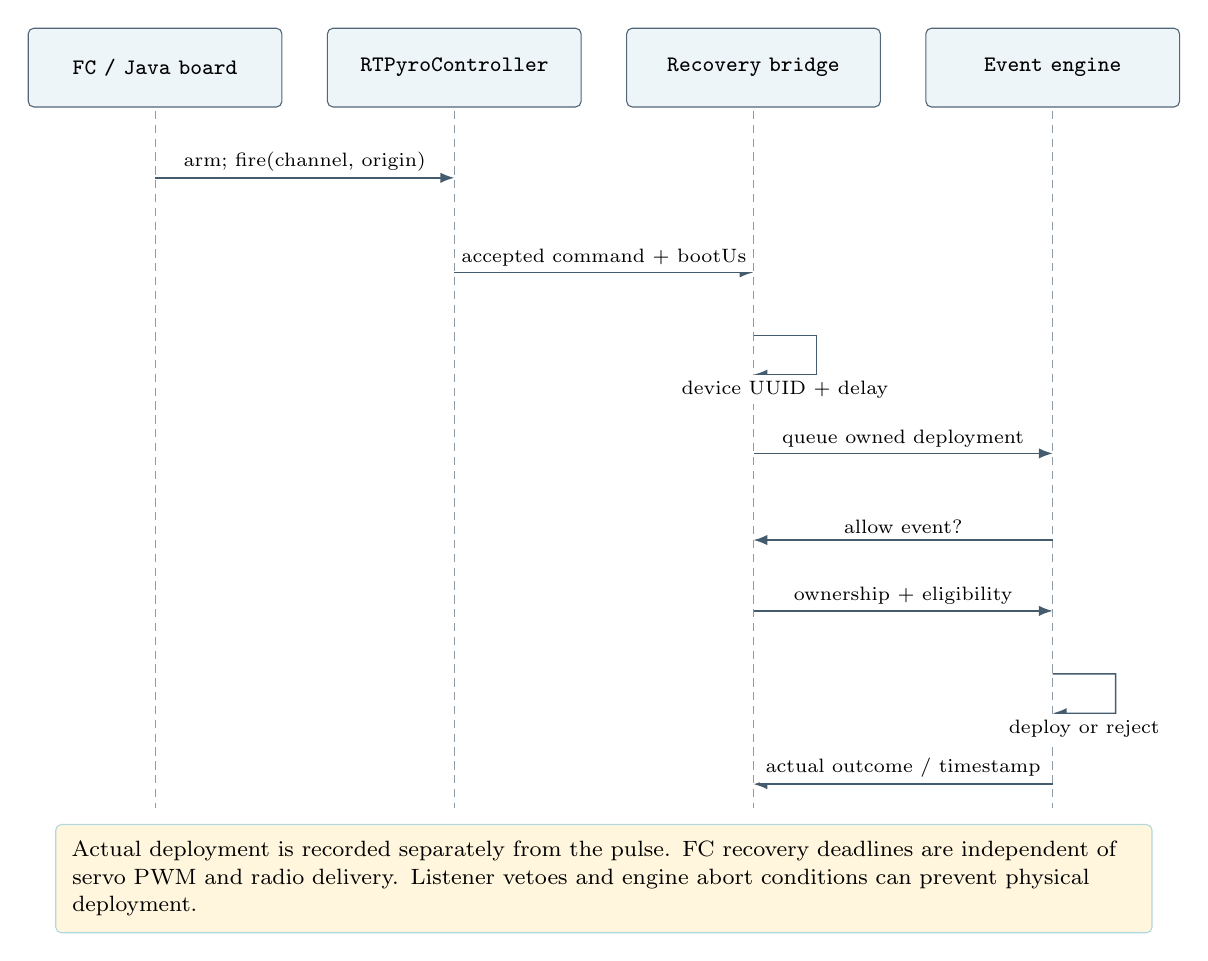
\begin{tikzpicture}
\node[participant,text width=2.8cm] at (1.5,0) {\ttfamily FC / Java board};
\node[participant,text width=2.8cm] at (5.3,0) {\ttfamily RTPyroController};
\node[participant,text width=2.8cm] at (9.1,0) {\ttfamily Recovery bridge};
\node[participant,text width=2.8cm] at (12.9,0) {\ttfamily Event engine};
\foreach \x in {1.5,5.3,9.1,12.9} \draw[lifeline] (\x,-0.55) -- (\x,-9.4);
\draw[use] (1.5,-1.4) -- node[flowlabel,above]{arm; fire(channel, origin)} (5.3,-1.4);
\draw[use] (5.3,-2.6) -- node[flowlabel,above]{accepted command + bootUs} (9.1,-2.6);
\draw[use] (9.1,-3.4) -- ++(0.8,0) -- ++(0,-0.5) -- node[flowlabel,below]{device UUID + delay} (9.1,-3.9);
\draw[use] (9.1,-4.9) -- node[flowlabel,above]{queue owned deployment} (12.9,-4.9);
\draw[use] (12.9,-6.0) -- node[flowlabel,above]{allow event?} (9.1,-6.0);
\draw[use] (9.1,-6.9) -- node[flowlabel,above]{ownership + eligibility} (12.9,-6.9);
\draw[use] (12.9,-7.7) -- ++(0.8,0) -- ++(0,-0.5) -- node[flowlabel,below]{deploy or reject} (12.9,-8.2);
\draw[use] (12.9,-9.1) -- node[flowlabel,above]{actual outcome / timestamp} (9.1,-9.1);
\node[note,text width=13.5cm] at (7.2,-10.3) {Actual deployment is recorded separately from the pulse. FC recovery deadlines are independent of servo PWM and radio delivery. Listener vetoes and engine abort conditions can prevent physical deployment.};
\end{tikzpicture}}

FC-enabled simulation overrides normal OpenRocket deployment rules. Those
saved rules resume when FC simulation is disabled. Physical deployment is
still subject to engine checks, listener vetoes and abort conditions, and is
recorded separately for logs, plots and canopy animation.

The firmware pulse expires using a strict elapsed-millisecond threshold
of more than \(250\ms\). Physical deployment scheduling retains the accepted
command's microsecond timestamp. Continuity affects firmware status reporting;
the \code{firePyro} acceptance gate itself checks arming rather than requiring
simulated continuity.

\clearpage
\section{Telemetry, logging and logical hardware}
\class{RTTelemetryEngine} preserves transmitted packet bytes and decodes them
to ground-station-compatible CSV. Received streams add deterministic packet
loss and delivery delay. \code{OR.log} contains action records and structured
physical/FC plot samples; metadata records paths, settings and completion.

\diagram{fig:telemetry}{Transmitted and received streams, plus the retained logical hardware adapters.}{%
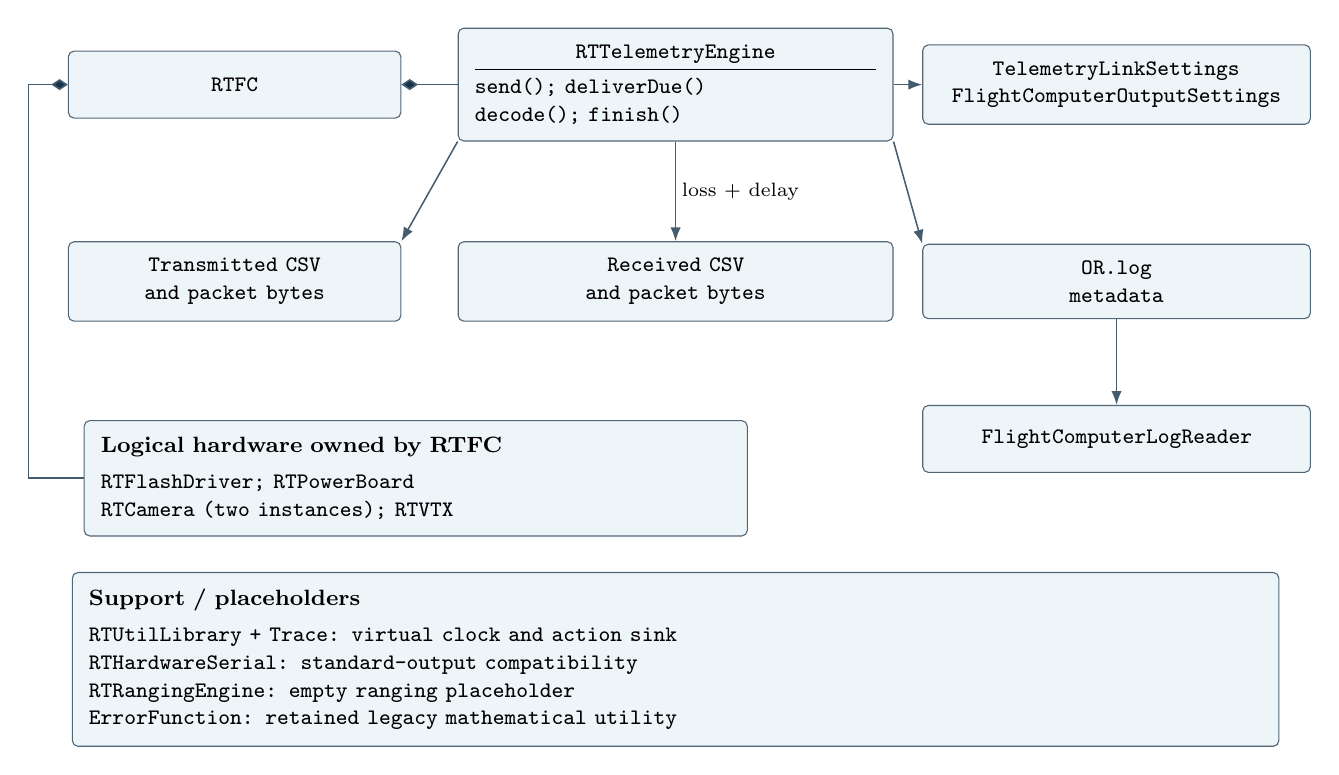
\begin{tikzpicture}
\simple{fc}{2.4,0}{RTFC}{3.8cm}
\uml{telem}{8,0}{RTTelemetryEngine}{send(); deliverDue()\\decode(); finish()}{5.1cm}
\simple{settings}{13.6,0}{TelemetryLinkSettings\\FlightComputerOutputSettings}{4.5cm}
\draw[own] (fc) -- (telem);
\draw[use] (telem) -- (settings);
\simple{tx}{2.4,-2.5}{Transmitted CSV\\and packet bytes}{3.8cm}
\simple{rx}{8,-2.5}{Received CSV\\and packet bytes}{5.1cm}
\simple{log}{13.6,-2.5}{OR.log\\metadata}{4.5cm}
\draw[use] (telem.south west) -- (tx.north east);
\draw[use] (telem) -- node[flowlabel,right]{loss + delay} (rx);
\draw[use] (telem.south east) -- (log.north west);
\simple{replay}{13.6,-4.5}{FlightComputerLogReader}{4.5cm}
\draw[use] (log) -- (replay);
\node[box,text width=8cm] (hardware) at (4.7,-5) {\textbf{Logical hardware owned by RTFC}\\[3pt]
\ttfamily RTFlashDriver; RTPowerBoard\\RTCamera (two instances); RTVTX};
\draw[own] (fc.west) -- ++(-0.5,0) |- (hardware.west);
\node[box,text width=14.9cm] at (8,-7.3) {\textbf{Support / placeholders}\\[3pt]
\ttfamily RTUtilLibrary + Trace: virtual clock and action sink\\
RTHardwareSerial: standard-output compatibility\\
RTRangingEngine: empty ranging placeholder\\
ErrorFunction: retained legacy mathematical utility};
\end{tikzpicture}}

Existing output files are protected against overwrite. Batch and ensemble
members receive distinct output paths. Telemetry is streamed, while result
branches retain plotted samples; short-period traces can still produce large
files. Downlink effects change ground observability, not the closed-loop
physical control calculation.

\class{FlightComputerLogReader} reconstructs available channels and actual
recovery events without executing custom Java from an imported file.
Camera/video, flash and power adapters expose logical operations or nominal
values. They do not model RF propagation, electronics, flash wear or battery
dynamics. The serial wrapper opens no physical serial port.

\clearpage
\section{Designer, persistence and custom programs}
\class{FlightComputerDesign} is the immutable JSON design and validation
boundary. \class{FlightComputerModels} defines hardware capabilities and
defaults. The standard library imports external \code{.fc} files, resolves
references and records behavior fingerprints, excluding presentation-only
names/layout from those fingerprints.

\diagram{fig:designer}{Portable FC definitions, simulation-specific assignments and the graphical editing/runtime connections.}{%
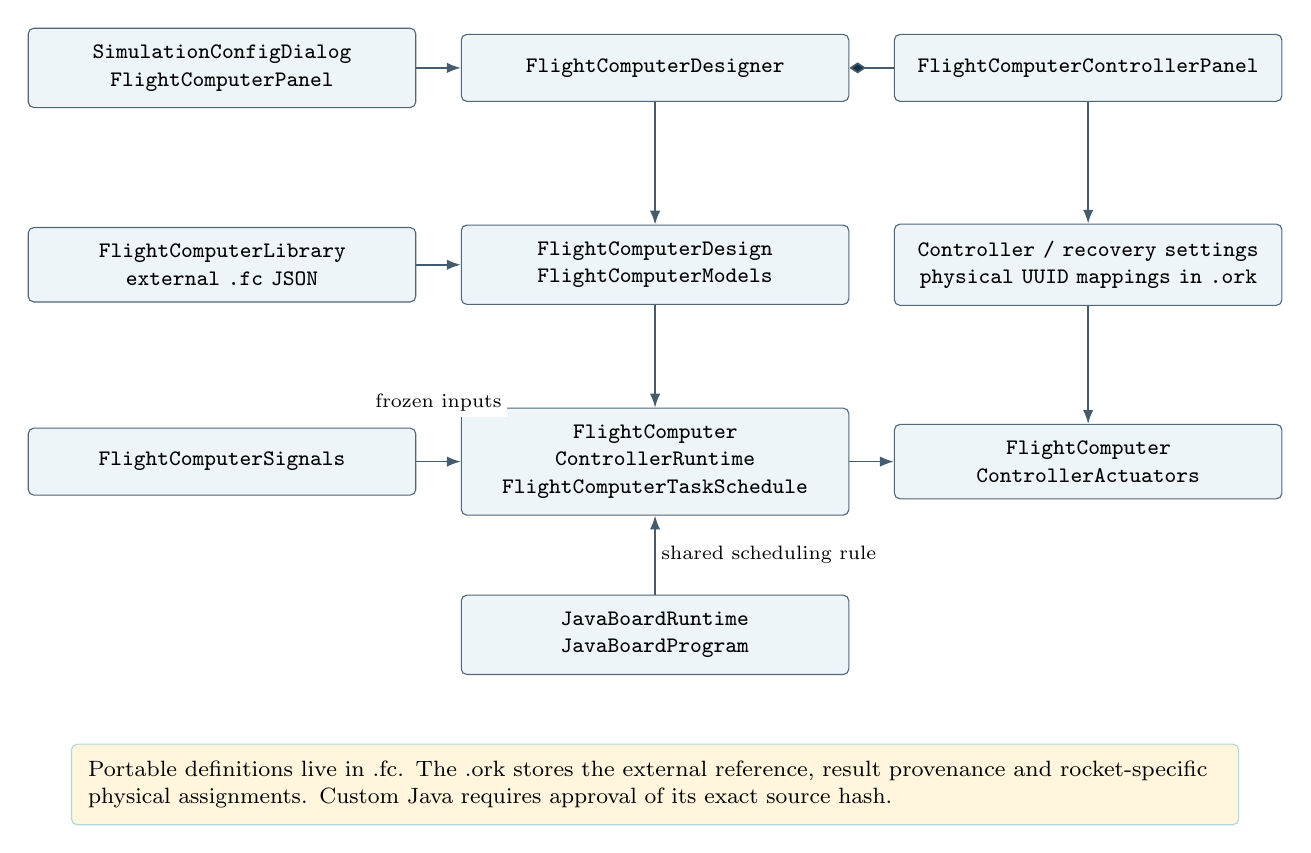
\begin{tikzpicture}
\simple{dialog}{2.5,0}{SimulationConfigDialog\\FlightComputerPanel}{4.5cm}
\simple{designer}{8,0}{FlightComputerDesigner}{4.5cm}
\simple{panel}{13.5,0}{FlightComputerControllerPanel}{4.5cm}
\draw[use] (dialog) -- (designer);
\draw[own] (designer) -- (panel);
\simple{library}{2.5,-2.5}{FlightComputerLibrary\\external .fc JSON}{4.5cm}
\simple{design}{8,-2.5}{FlightComputerDesign\\FlightComputerModels}{4.5cm}
\simple{mapping}{13.5,-2.5}{Controller / recovery settings\\physical UUID mappings in .ork}{4.5cm}
\draw[use] (designer) -- (design);
\draw[use] (library) -- (design);
\draw[use] (panel) -- (mapping);
\simple{signal}{2.5,-5.0}{FlightComputerSignals}{4.5cm}
\simple{runtime}{8,-5.0}{FlightComputer\\ControllerRuntime\\FlightComputerTaskSchedule}{4.5cm}
\simple{actuators}{13.5,-5.0}{FlightComputer\\ControllerActuators}{4.5cm}
\draw[use] (design) -- (runtime);
\draw[use] (signal) -- node[flowlabel,above=16pt]{frozen inputs} (runtime);
\draw[use] (runtime) -- (actuators);
\draw[use] (mapping) -- (actuators);
\simple{java}{8,-7.2}{JavaBoardRuntime\\JavaBoardProgram}{4.5cm}
\draw[use] (java) -- node[flowlabel,right]{shared scheduling rule} (runtime);
\node[note,text width=14.4cm] at (8,-9.1) {Portable definitions live in .fc. The .ork stores the external reference, result provenance and rocket-specific physical assignments. Custom Java requires approval of its exact source hash.};
\end{tikzpicture}}

The simulation's Flight computer tab opens the designer. Hardware, behavior,
Java and controller editors apply snapshot changes with undo/redo. Controller
editing combines algorithm settings, measured-source/quantity selection,
baselines, tuning, timing, states and eligible physical targets.

Custom source derives from \class{JavaBoardProgram}; each run creates fresh
instances. Compilation does not initialize the program class. Execution
requires local approval of the exact source hash and occurs inside the
OpenRocket process, without a sandbox. Independently scheduled boards run
in tandem for algorithm experiments, but do not provide an authoritative
model of inter-board communications.

\clearpage
\section{Results and adjacent simulation improvements}
\class{FlightComputerData} and \class{FlightComputerControllerPlots} record
measured/physical comparisons, servo outputs, controller diagnostics and state.
Digital commands/status use held-value plotting. Structured log metadata
preserves channel identities and units during import.

\diagram{fig:results}{Result paths for FC diagnostics, trajectory animation, ensemble statistics and motor searches.}{%
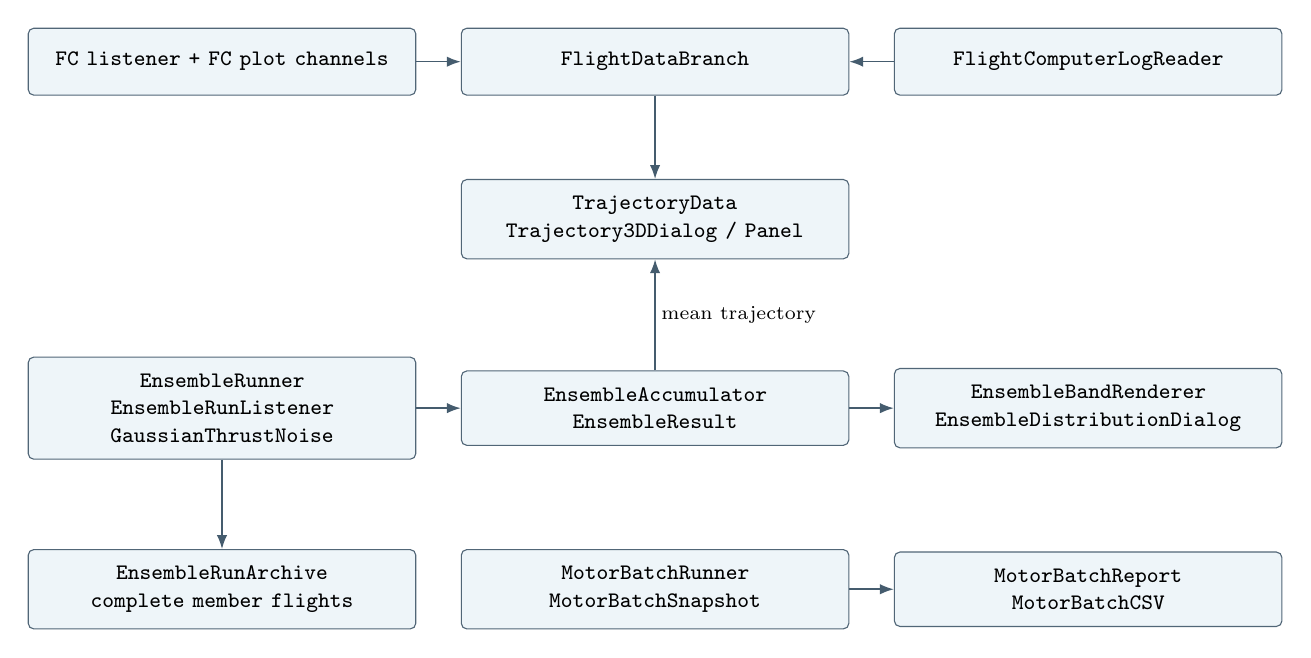
\begin{tikzpicture}
\simple{fc}{2.5,0}{FC listener + FC plot channels}{4.5cm}
\simple{branch}{8,0}{FlightDataBranch}{4.5cm}
\simple{replay}{13.5,0}{FlightComputerLogReader}{4.5cm}
\draw[use] (fc) -- (branch);
\draw[use] (replay) -- (branch);
\simple{trajectory}{8,-2}{TrajectoryData\\Trajectory3DDialog / Panel}{4.5cm}
\draw[use] (branch) -- (trajectory);
\simple{runs}{2.5,-4.4}{EnsembleRunner\\EnsembleRunListener\\GaussianThrustNoise}{4.5cm}
\simple{stats}{8,-4.4}{EnsembleAccumulator\\EnsembleResult}{4.5cm}
\simple{plots}{13.5,-4.4}{EnsembleBandRenderer\\EnsembleDistributionDialog}{4.5cm}
\draw[use] (runs) -- (stats);
\draw[use] (stats) -- (plots);
\draw[use] (stats) -- node[flowlabel,right]{mean trajectory} (trajectory);
\simple{archive}{2.5,-6.7}{EnsembleRunArchive\\complete member flights}{4.5cm}
\draw[use] (runs) -- (archive);
\simple{batch}{8,-6.7}{MotorBatchRunner\\MotorBatchSnapshot}{4.5cm}
\simple{report}{13.5,-6.7}{MotorBatchReport\\MotorBatchCSV}{4.5cm}
\draw[use] (batch) -- (report);
\end{tikzpicture}}

\class{TrajectoryData} reconstructs position, recorded quaternion orientation,
motor burns and recovery events. The cartoon attitude follows that orientation,
not velocity direction. Actual deployment controls the canopy, burn intervals
control exhaust, and FC state labels follow the playhead.

Ensemble engine variation is additive:
\begin{equation}
 T_{\mathrm{member}}(t)=\max\{0,\,T(t)+e(t)\},
 \qquad e(t)\text{ is the configured Gaussian perturbation during burn}.
\end{equation}
Configured atmospheric variation is applied separately. Members are aligned
in physical time to form the mean and sample standard deviation. 2D plots
show mean \(\pm1\sigma\); 3D uses the mean trajectory. Scalar distributions
use each member's extrema/metrics, and the archive retains complete flights.

Motor-batch workers use isolated baseline snapshots, record candidate/delay
outcomes and export CSV. Update and memory helpers are documented maintenance
utilities, rather than FC runtime dependencies.

\clearpage
\section{Complete firmware class index}
All entries below are beneath \code{edu.mit.rocket_team}. The generated
Javadoc gives the complete method-level API, including private members.
The index includes legacy and placeholder classes so their presence is not
mistaken for active physical hardware simulation.

\small
\begin{longtable}{@{}>{\raggedright\arraybackslash}p{5.65cm}>{\raggedright\arraybackslash}p{2.1cm}>{\raggedright\arraybackslash}p{7.4cm}@{}}
\toprule Class & Subpackage & Responsibility\\\midrule
\endfirsthead
\toprule Class & Subpackage & Responsibility (continued)\\\midrule
\endhead
\bottomrule
\endfoot
\class{RTCamera} & \code{AV} & Logical camera setup; two instances are owned by the FC.\\
\class{RTVTX} & \code{AV} & Logical video-transmitter power requests.\\
\class{FlightComputerTimingSettings} & \code{FC} & Read/work/jitter costs, PWM phase and timing seed.\\
\class{RTFC} & \code{FC} & Translated sketch, loop phases, state actions and PWM snapshots.\\
\class{RTPyroController} & \code{control} & Six-channel arm/fire, pulse and status logic.\\
\class{RTRollController} & \code{control} & Firmware roll PID and aerodynamic gain schedule.\\
\class{RTAirbrakesAccelerationMeasurement} & \code{control.}\newline\code{airbrakes} & Acceleration/time sample for the coast fit.\\
\class{RTAirbrakesController} & \code{control.}\newline\code{airbrakes} & Included coast predictor and airbrake control sequence.\\
\class{RTAirbrakesControllerState} & \code{control.}\newline\code{airbrakes} & Predictor preparation and control phase enumeration.\\
\class{RTAirbrakesVelocityMeasurement} & \code{control.}\newline\code{airbrakes} & Velocity/time sample for the coast fit.\\
\class{RTAccel} & \code{instrument} & Fresh-sample consumption and longitudinal velocity integration.\\
\class{RTBaro} & \code{instrument} & Pressure altitude, moving average, zeroing and maximum tracking.\\
\class{RTGPS} & \code{instrument} & Held GPS fix, quantization, relative height and maximum tracking.\\
\class{RTGyro} & \code{instrument} & Angular-rate integration and firmware attitude conventions.\\
\class{RTMag} & \code{instrument} & Legacy magnetometer/roll injection adapter.\\
\class{RTFlashDriver} & \code{internal} & Logical logging allocation and packet append operations.\\
\class{RTPowerBoard} & \code{internal} & Nominal power values, converter enables and protection flags.\\
\class{FlightComputerOutputSettings} & \code{telemetry} & CSV/log paths and distinct multi-run filenames.\\
\class{RTRangingEngine} & \code{telemetry} & Reserved empty ranging placeholder.\\
\class{RTTelemetryEngine} & \code{telemetry} & Byte queues, loss/delay, packet decoding and streamed files.\\
\class{TelemetryLinkSettings} & \code{telemetry} & Reproducible downlink configuration.\\
\pagebreak
\class{ErrorFunction} & \code{util} & Legacy error-function and normal-distribution approximations.\\
\class{RTController} & \code{util} & Common setup, loop and injection interface for controllers.\\
\class{RTInstrument} & \code{util} & Instrument base sharing the run-local clock and trace.\\
\class{RTRocketState} & \code{util} & Firmware phase codes used by commands and telemetry.\\
\class{RTSimulationCommunicator} & \code{util} & Latched commands to per-run airbrakes and tab fins.\\
\class{RTUtilLibrary} & \code{util} & Unsigned clock arithmetic, nested Trace and orientation helpers.\\
\class{RTAccelData} & \code{util.data} & Mutable sensor-axis specific-force payload.\\
\class{RTBaroData} & \code{util.data} & Barometer engineering values and optional raw ADC fields.\\
\class{RTFudgedAirbrakesData} & \code{util.data} & Legacy predictor altitude/velocity/acceleration/apogee inputs.\\
\class{RTFudgedData} & \code{util.data} & Shared marker base for injected payloads.\\
\class{RTGPSData} & \code{util.data} & Coordinates, MSL altitude, fix and dilution-of-precision values.\\
\class{RTGyroData} & \code{util.data} & Mutable angular-rate payload.\\
\class{RTMagData} & \code{util.data} & Legacy magnetometer and supplied roll payload.\\
\class{RTPyroStatus} & \code{util.data} & Two-bit firmware continuity/firing status enumeration.\\
\class{RTHardwareSerial} & \code{util.}\newline\code{hardware} & Standard-output compatibility for firmware serial calls.\\
\end{longtable}
\normalsize

\clearpage
\section{Build, regeneration and verification}
The code scope and context classes are defined by two manifests within the
Gradle project:
\begin{lstlisting}
config/mit-documentation-sources.txt
config/mit-javadoc-connectors.txt
\end{lstlisting}
From \code{clone/openrocket-release-24.12.RC.01}, with JDK 17:
\begin{lstlisting}[language=bash]
./gradlew formatMitJava
./gradlew verifyMitJavadoc rocketTeamJavadoc
./gradlew shadowJar
\end{lstlisting}
Run formatting before compilation or documentation generation, not
concurrently. The formatter is pinned to google-java-format 1.24.0 with
four-space indentation and preservation of import order, unused imports and
string literals. Documentation dependencies are developer-only.

\code{verifyMitJavadoc} uses the JDK parser to audit every explicit method and
constructor in the improvement manifest, including private methods, test
helpers and anonymous callbacks. It fails on a missing description.
\code{rocketTeamJavadoc} includes private members and selected engine types,
and checks comment syntax and links. Missing field descriptions in upstream
classes are excluded from warnings; the separate method audit is not disabled.

\subsection{Compiling this entirely LaTeX report}
This file contains all prose, equations, tables and nine TikZ figures. There
are no external image inputs, shell-escape requirements or PlantUML dependencies.
From \code{doc/improvements}:
\begin{lstlisting}[language=bash]
latexmk -pdf -interaction=nonstopmode \
  -halt-on-error 14-flight-computer-api-and-architecture.tex
\end{lstlisting}
A normal LaTeX distribution with TikZ, Latin Modern, hyperref, listings,
booktabs, longtable and the packages listed in the preamble is sufficient.
The existing Markdown guide and its \code{rocketTeamUml} SVG generation task
remain separate companion documentation. This report's figures are edited
in the TikZ source, not regenerated from those SVGs.

\subsection{Recorded validation results}
\begin{itemize}
\item \textbf{1,560/1,560 explicit methods and constructors documented} across
150 original improvement files and the new parser/audit utility.
\item \textbf{150/150 original scoped files} retain their executable Java
tokens after comment/spacing removal and namespace normalization.
\item \textbf{148 core tests and 65 Swing/UI tests passed}, with no failures,
errors or skipped tests. Coverage includes firmware replay, microsecond
scheduling, PWM ties, recovery, independent actuators, controller blocks,
ensembles, motor batches, plots, editor lifetime and update routing.
\item \textbf{Root shadow JAR rebuilt successfully}. The startup class and
\code{edu/mit/rocket_team/FC/RTFC.class} are present; no entries remain beneath
the old namespace.
\item \textbf{Javadoc generated successfully} with documentation/link checks.
All 36 top-level firmware classes are represented by this report's figures
and complete class index.
\end{itemize}

Application artifact: \code{build/libs/OpenRocket-MIT-v6.4.jar}, with its
checksum and installed-app compatibility alias. Restart an already-running
application to load the renamed classes.

\clearpage
\section{Source map and limits of the model}
The main integration entry points, relative to the Gradle project, are:
\begin{lstlisting}
core/src/main/java/edu/mit/rocket_team/
core/src/main/java/info/openrocket/core/simulation/
  listeners/FlightControllerSimulatorListener.java
  extension/impl/ZephyrusFlightComputer.java
  flightcomputer/
swing/src/main/java/info/openrocket/swing/gui/
  flightcomputer/
  simulation/FlightComputerPanel.java
\end{lstlisting}
The connected framework types include \class{Simulation}, the two event
engines, \class{SimulationStatus}, \class{SimulationConditions},
\class{SimulationOptions}, the stepper/listener interfaces and helpers,
\class{FlightDataBranch}, \class{FlightEvent}, \class{FinSetCalc}, controlled
fins, airbrakes and \class{RecoveryDevice}.

\begin{table}[htbp]\centering\small
\begin{tabularx}{\linewidth}{@{}p{3.7cm}Y@{}}\toprule
Area & What the implementation establishes\\\midrule
Virtual scheduling & Deterministic ordering, acquisition age, completion delay and PWM/recovery deadlines for the configured model.\\
Processor and buses & User-supplied execution costs; no authoritative shared-CPU or inter-board communications model.\\
Sensors & Engineering-unit acquisition, noise/bias, rotation and firmware filtering; not complete sensor electronics.\\
Servos and aerodynamics & Commands reach physical fin/airbrake models; no modeled servo dynamics or general qualification of high-deflection aerodynamics.\\
Recovery & Accepted logical commands connect to actual engine deployment events, subject to eligibility and abort rules.\\
Radio and power & Packet loss/delay and logical/nominal hardware behavior; not RF, battery or electrical dynamics.\\
\bottomrule\end{tabularx}
\caption{Implementation contracts and their practical limits.}
\end{table}

\subsection{Companion documents}
Within \code{doc/improvements}, the recovery implementation is described in
\code{11-flight-computer-recovery-implementation.md}; controller behavior,
ownership, tuning and verification are described in
\code{13-flight-computer-controller-implementation.md}. The browsable method
reference begins at \code{javadoc/index.html}.

Repository: \href{https://github.com/MDNich/ActiveControl_MIT_RktTeam}{github.com/MDNich/ActiveControl\_MIT\_RktTeam}.
The report describes the 6.4 implementation verified on 11 October 2026.
Diagrams are curated architecture views and must be updated when source
relationships or scheduling order change.
\end{document}
